\documentclass[final,inline,a4paper,narroweqnarray]{ieee}
% In order to use the figure-defining commands in ieeefig.sty...
\usepackage{ieeefig}
% To use utf8 encoding
\usepackage[T1]{fontenc}
\usepackage[utf8]{inputenc}
\usepackage[spanish]{babel}
% to place figures
\usepackage{float}
\usepackage{graphicx}
\usepackage{amsmath}
% dont use geometry package
%\usepackage{geometry}

% "hack" to place figures in subsection
\usepackage{placeins}
\let\Oldsection\section
\renewcommand{\section}{\FloatBarrier\Oldsection}
\let\Oldsubsection\subsection
\renewcommand{\subsection}{\FloatBarrier\Oldsubsection}
\let\Oldsubsubsection\subsubsection
\renewcommand{\subsubsection}{\FloatBarrier\Oldsubsubsection}

\begin{document}

%----------------------------------------------------------------------
% Title Information, Abstract and Keywords
%----------------------------------------------------------------------
\title[TP N$^o$ 2: Rutas en Internet]{%
Trabajo Práctico N$^o$ 2: Rutas en Internet}

% format author this way for journal articles.
\author[Barrios, Benegas, Caravario, Rodriguez]{%
	Leandro Ezequiel Barrios,
	\and
	Gonzalo Benegas,
	\and
	Martin Caravario,
	\and
	Pedro Rodriguez
}

% make the title
\maketitle

% do the abstract
\begin{abstract}

En el presente Trabajo Práctico nos propondremos experimentar con herramientas 
y técnicas frecuentemente utilizadas a nivel de red. En particular, nos centraremos en la utilización de \texttt{traceroute} como herramienta para medir tiempos y \texttt{RTTS}. 

\end{abstract}

% start the main text ...

%----------------------------------------------------------------------
% SECTION I: Introduction
%----------------------------------------------------------------------
\section{Introducción}

Los objetivos del presente Trabajo Práctico son múltipes: por un lado, entender 
los protocolos involucrados en cada comunicación o intercambio de datos entre un 
usuario y un servidor, estando ambos conectados a Internet. Vimos en clase que 
estos protocolos son tanto de nivel de capa de transporte (TCP, UDP) como de 
aplicación (DNS, SMTP). Por otro lado, para afianzar nuestros conocimientos, 
implementaremos una herramienta que cumpla la misma función que 
\texttt{traceroute} por nuestra cuenta. La función de esta herramienta es 
la de detectar, a partir del nombre de un dominio (host), cada uno de los 
nodos intermedios por los que pasa el paquete antes de llegar a la dirección
IP correspondiente a dicho host. En este TP, analizaremos los
RTT de paquetes enviados a distintas universidades del mundo. 


%----------------------------------------------------------------------
% SECTION II: Caracterizando Rutas
%----------------------------------------------------------------------
\section{Caracterizando Rutas}

  %----------------------------------------------------------------------
  %  SUBSECTION III: Implementación de tool para hacer traceroute
  %----------------------------------------------------------------------
  \subsection{Implementación de tool para hacer traceroute}
  Implementamos la herramienta \texttt{traceroute2} en python, usando la librería
  \emph{scapy}. Para esto, armamos varios paquetes echo-request, inicianizándolos con un TTL
  entre 1 y alguna cantidad de hops variable, que nos permita llegar al destino (en
  general, 30 o 40 hops son más que suficientes). A cada paquete ICMP que es respondido,
  le corresponderá un RTT diferente y, los paquetes que no son respondidos después de un tiempo
  de timeout determinado, asumimos que fueron recibidos y no respondidos o que se perdieron en la red,
  marcando que el RTT y resto de la información correspondiente a dicho paquete con un $*$. \\
  Una herramienta extra que implementamos para facilitar la experimentación
  fue una función que llamamos DNSInverso, que para cada router nos permite reconocer su nombre.
  De esta forma podemos detectar, para cada máquina de la que obtenemos respuesta en algún hop,
  a qué organización pertenece (si es que pertenece a alguna). Y, en particular,
  si pertenece a la universidad a la que estamos haciendo el traceroute.
  
  A partir de los valores de RTT obtenidos para cada nodo intermedio de la ruta rastreada por
  \texttt{traceroute2}, graficamos el RTT observado entre dicho nodo y el nodo origen.

  %----------------------------------------------------------------------
  %  SUBSECTION III: Adaptación de la tool
  %----------------------------------------------------------------------
  \subsection{Adaptación de la tool}
  Después de haber experimentado con la tool original, enviando paquetes
  echo-request a varias universidades alrededor del mundo, 
  adaptamos dicha \emph{tool} para que, una vez terminada 
  la búsqueda, calcule el \emph{valor standard}  o \emph{valor Z (ZRTT) } 
  en cada salto con respecto a los saltos realizados en la ruta global de la 
  siguiente manera: si $RTT_i$ 
  es el RTT medido para el salto $i$, se define $ ZRTT_i = \dfrac{RTT_i 
  - \overline{RTT}}{SRTT} $ donde $\overline{RTT}$ y $SRTT$ son el promedio 
  y el desvío estandard de una lista que contiene las diferencias de RTT entre
  cada hop y el hop que lo antecede en la ruta que realiza el paquete.
  
  Luego, para cada hop $i$ tendremos un valor $|ZRTT_i|$. Por cómo definimos a $ZRTT_i$, 
  se observa que a mayor $valor Z$ para un hop, mayor será la variación del tiempo que se
  tarda en atravesar dicho hop en comparación con el promedio del tiempo que se tarda 
  en atravesar cada hop de la ruta.

  A partir de esta adaptación esperamos introducir en los gráficos de RTT = f(número de hop) 
  que habíamos hecho con la $tool$ original la nueva información obtenida sobre cada hop.
  Esperamos que esto nos permita detectar aquellos hops que corresponden a enlaces submarinos. 
  En particular, si el hop $i$ tiene un $|ZRTT_i|$ mucho mayor que el resto, sería un indicator
  de que en el hop $i$ el paquete atraviesa un enlace submarino. 

%----------------------------------------------------------------------
% SECTION III: Traceroute a universidades del mundo
%----------------------------------------------------------------------
\section{Experimentación: Traceroute a universidades del mundo}

A partir de la herramienta \texttt{traceroute2} y tomando como IP origen la de la PC de uno de los integrantes del grupo,
realizamos rastreos para distintas universidades alrededor del mundo. Cada una de estas universidades las identificamos
a partir de su URL correspondiente. 
En el proceso de la experimentación, introdujimos los datos obtenidos para cada universidad en un graficador, que 
dada la lista de direcciones IP recorridas, las localiza geográficamente en un mapa del planeta Tierra, 
y las une mediante una línea.

Las universidades que terminamos eligiendo fueron: en Noruega (Oslo) a <<www.uio.no>>, en 
Japón (Tokyo) a <<www.u-tokyo.ac.jp>>, en Tanzania (Dar es Salaam) a <<www.udsm.ac.tz>> y 
en Nueva Zelanda (Auckland) a <<www.auckland.ac.nz>>. 

De esta forma, intentamos expresar de la forma más gráfica posible el camino a 
escala global que debió efectuar cada paquete para llegar desde nuestra PC hasta algún servidor de dicha universidad, 
ubicada a decenas de miles de kilómetros de nosotros. 

Uno de los problemas con que nos encontramos encontrar universidades para las cuáles los trayectos efectuados por los paquetes 
tuvieran distintas características topológicas (por ejemplo que los paquetes atraviesen enlaces submarinos o que
las universidades queden en distintos continentes), a fin 
de poder realizar posteriormente un análisis más completo e interesante de los RTTs y ZRTTs
correspondientes a cada trayectoria.  

Dos de los problemas con los que nos encontramos durante la experimentación fueron:
\begin{itemize}
	\item tuvimos problemas con el envío de paquetes a través de conexión wi-fi. Es por 
	esto que tuvimos que realizar todas las mediciones con una misma computadora, 
	conectada a internet a través de una conexión cableada.
	\item encontramos muchas universidades, como por ejemplo la de Nairobi (www.uombi.ac.ke), 
	para las cuáles el camino graficado en el mapa terminaba en EEUU, en lugar de de en África, 
	como esperábamos. Para estos
	casos, supusimos que el problema no era de un bug en nuestra implementación, sino en que
	dicha página web estaba hosteada
	en un servidor localizado en EEUU. Una posible razón por la cuál dicha universidad 
	querría hacer esto podría ser, por 
	ejemplo, que el costo de hostear un servidor en Kenia es mayor que en EEUU.
	\item en todos los casos analizados, hubieron muchos nodos intermedios que no 
	contestaban nuestro \emph{ICMP Request}, con
	lo cuál habían muchos \emph{hops} que no éramos capaces de localizar en el mapa, 
	lo cuál restaba precisión a nuestra 
	representación de la trayectoria de los paquetes.
	\item hubieron algunas universidades para las cuáles (por ejemplo, al enviar
	40 paquetes a www.udsm.ac.tz) había un primer router localizado en dicha universidad  
	nos contestaba, pero
	después de obtener esta respuesta, dejábamos de obtener respuesta. De esta forma, no 
	logramos obtener una respuesta de la IP destino. Creemos quue este 
	último router que nos contestaba estaba actuando como firewall de la red interna
	de dicha universidad.
\end{itemize}

\subsection{Gráficos y análisis}

\subsubsection{Universidad de Auckland}
\begin{figure}[ht]\begin{center}
   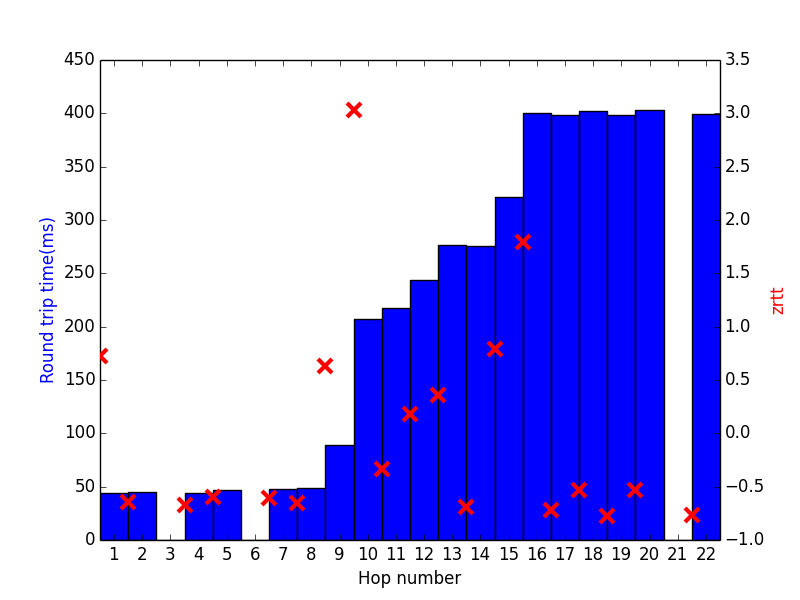
\includegraphics[width=0.5\textwidth]{%
    imagenes/auckland.png}
    \caption{Auckland}
    \label{Auckland}
\end{center}\end{figure}

\begin{figure}[ht]\begin{center}
   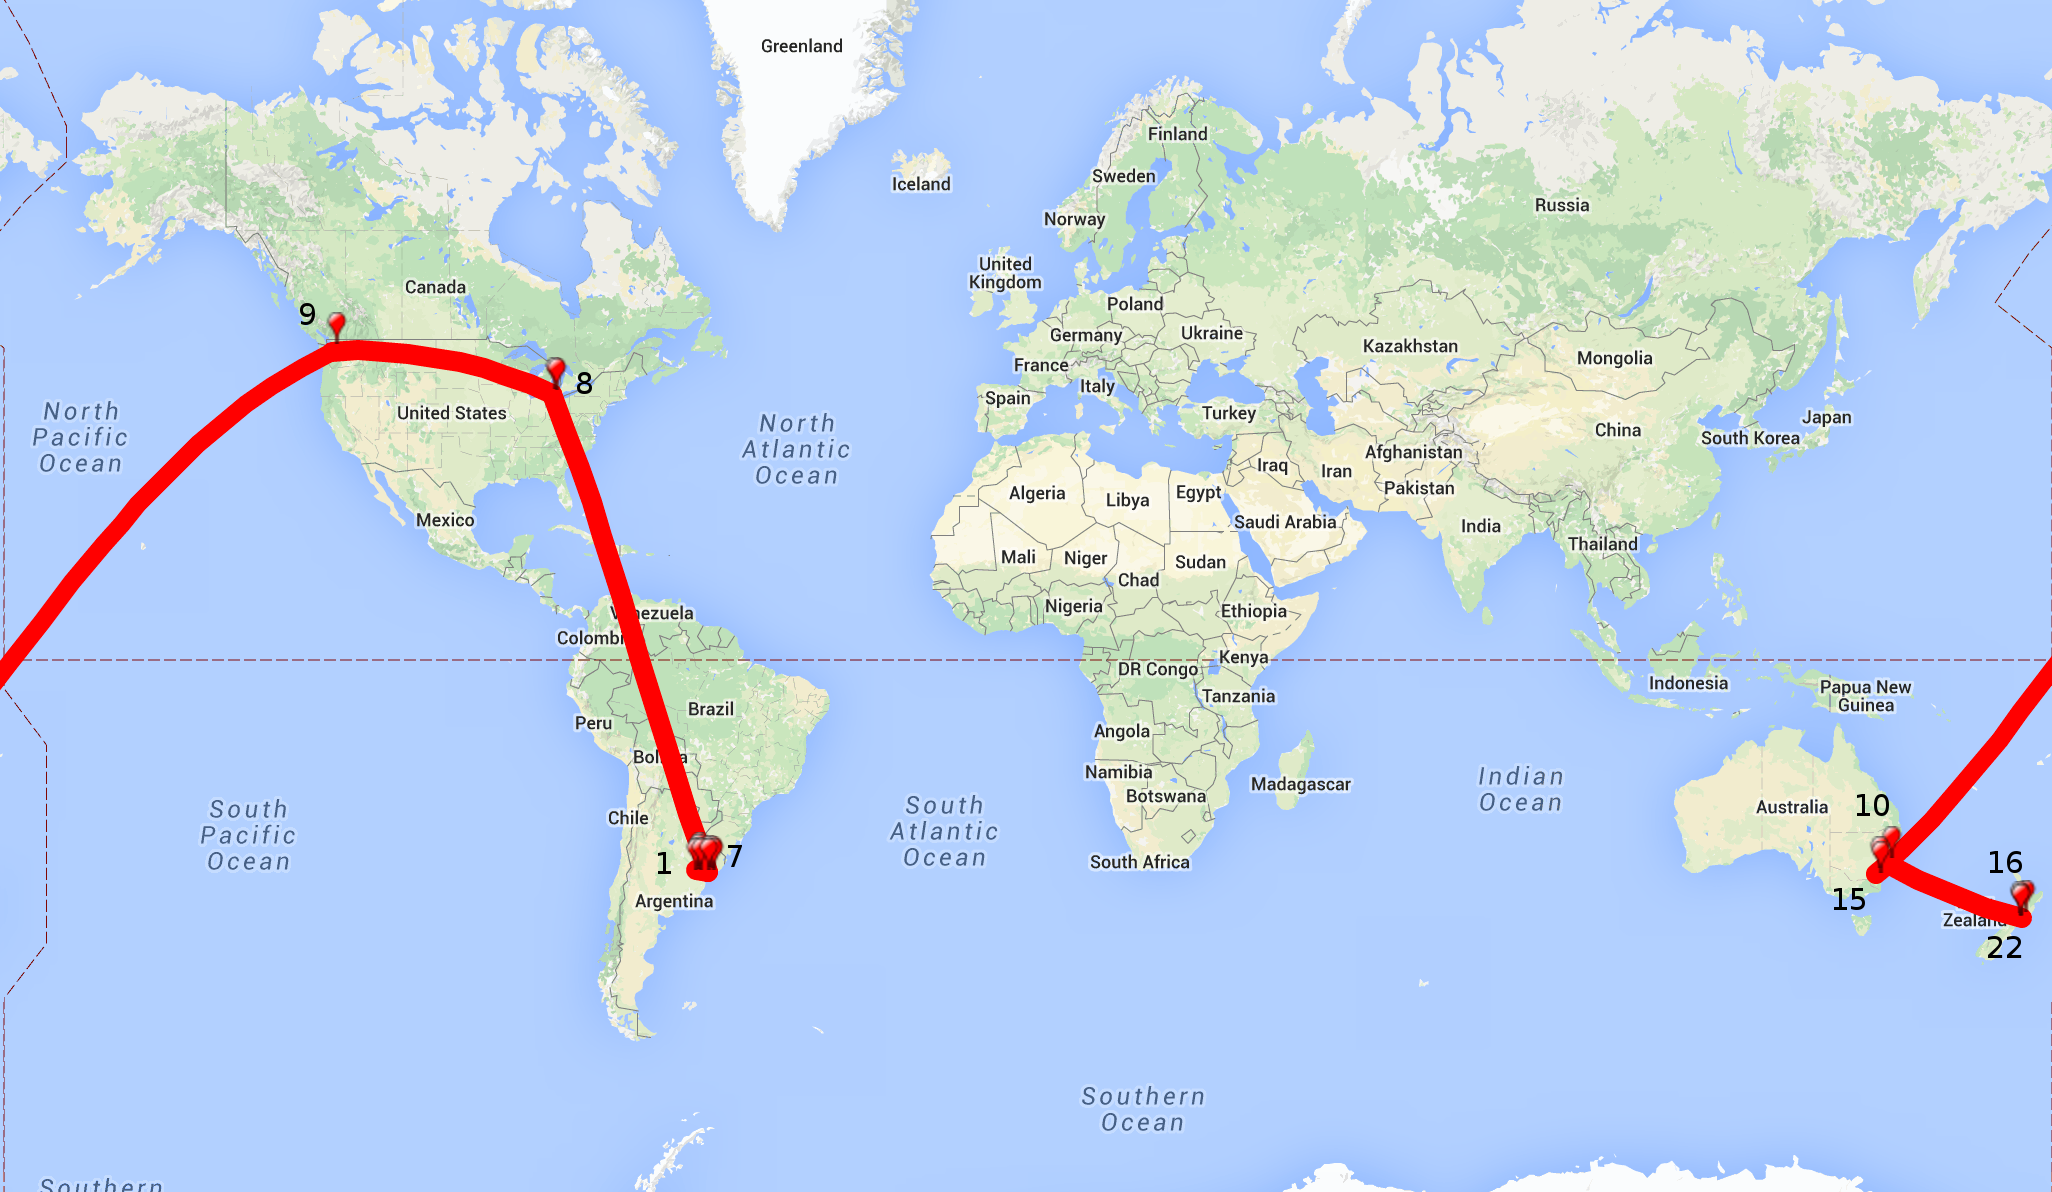
\includegraphics[width=0.5\textwidth]{%
    imagenes/auckland-mapa.png}
    \caption{Auckland - mapa}
    \label{Auckland}
\end{center}\end{figure}

\subsubsection{Universidad de Tanzania}
\begin{figure}[ht]\begin{center}
   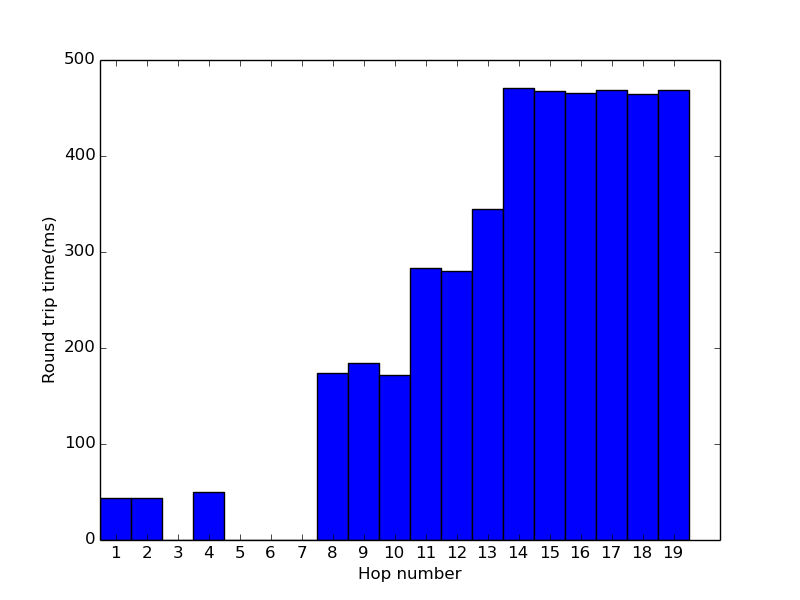
\includegraphics[width=0.5\textwidth]{%
    imagenes/tanzania.png}
    \caption{Tanzania}
    \label{Tanzania}
\end{center}\end{figure}

\begin{figure}[ht]\begin{center}
   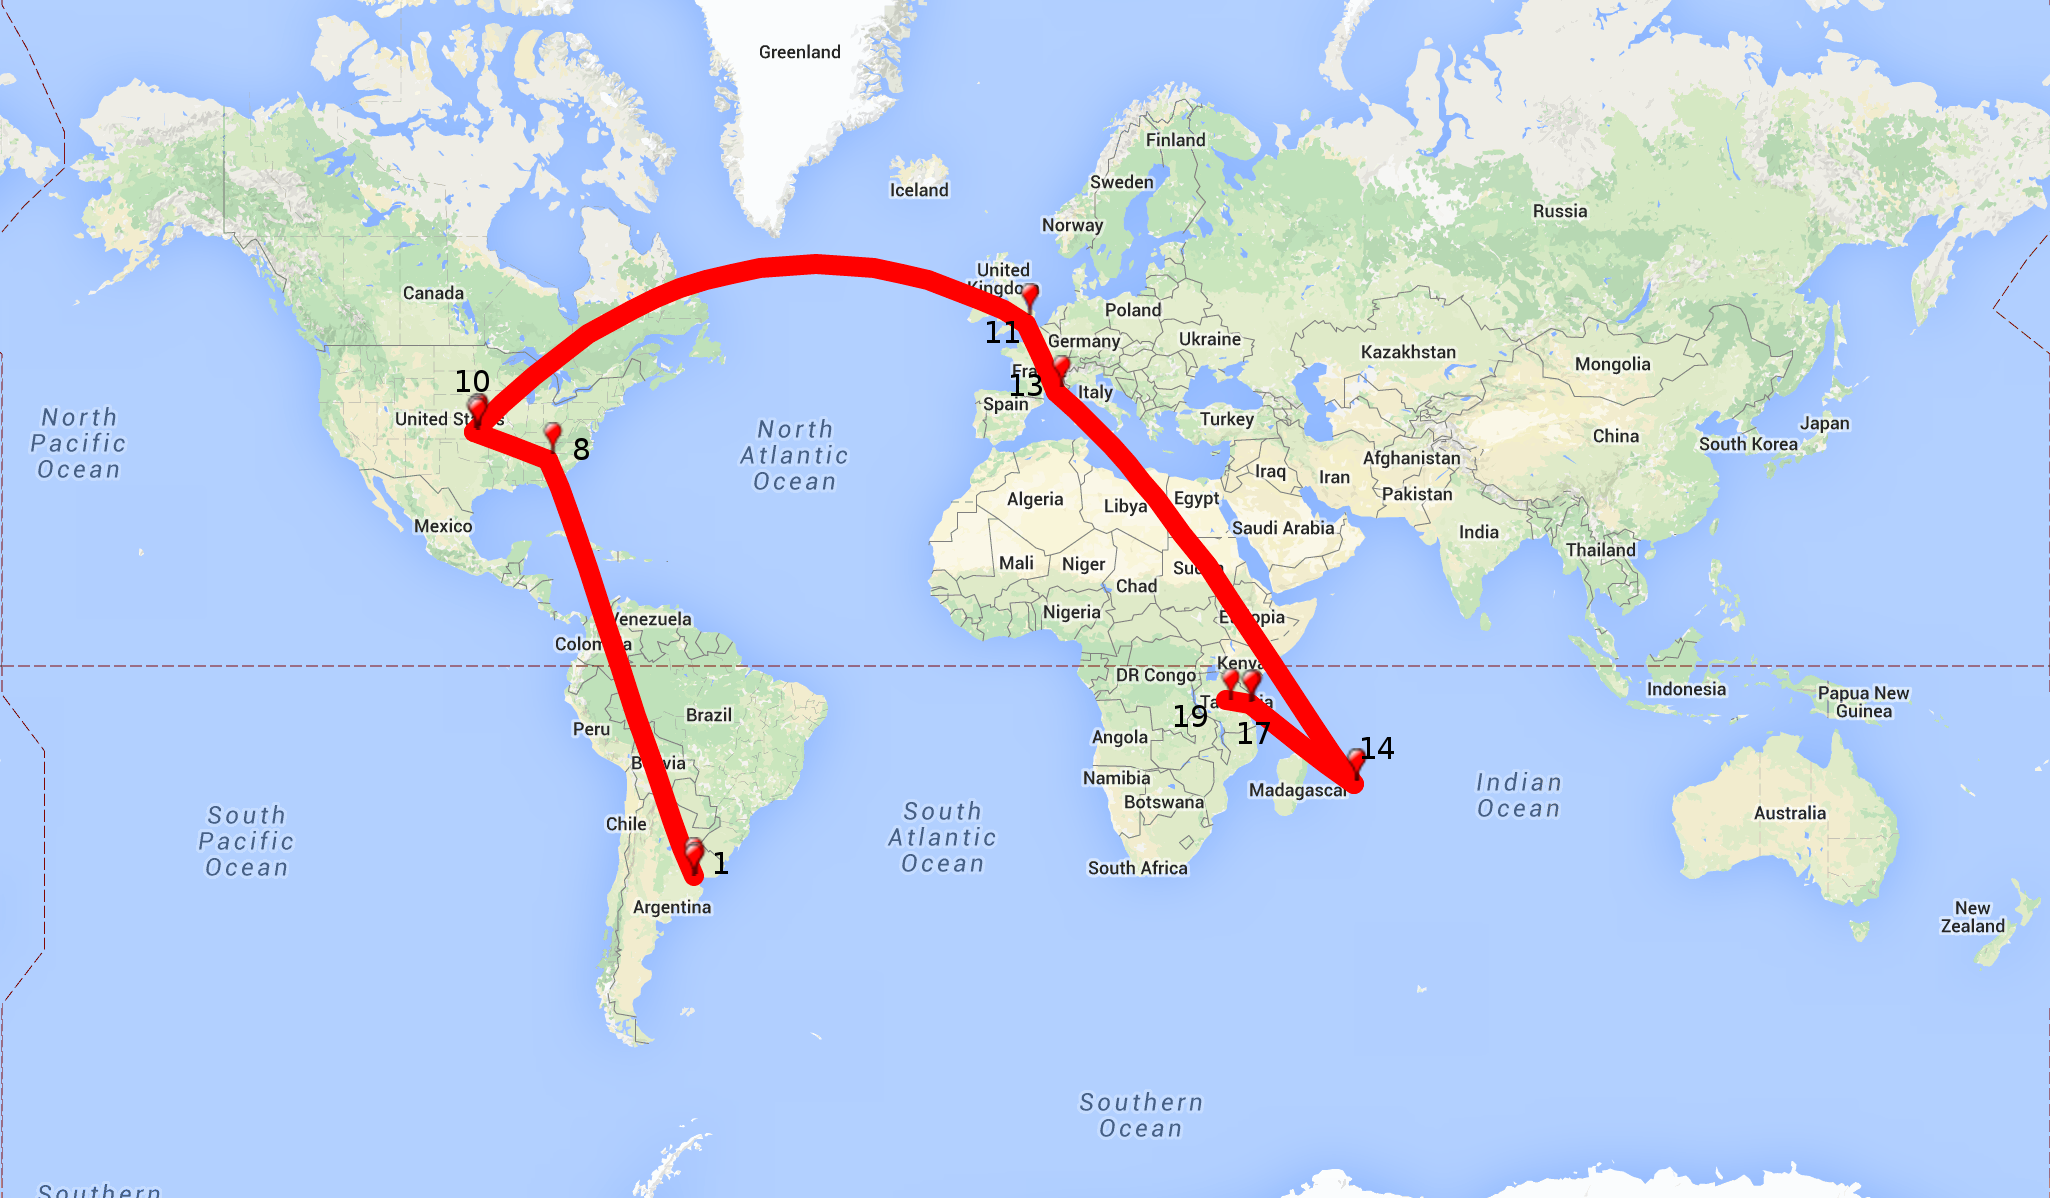
\includegraphics[width=0.5\textwidth]{%
    imagenes/tanzania-mapa.png}
    \caption{Tanzania - mapa}
    \label{Tanzania}
\end{center}\end{figure}

\subsubsection{Universidad de Tokyo}
\begin{figure}[ht]\begin{center}
   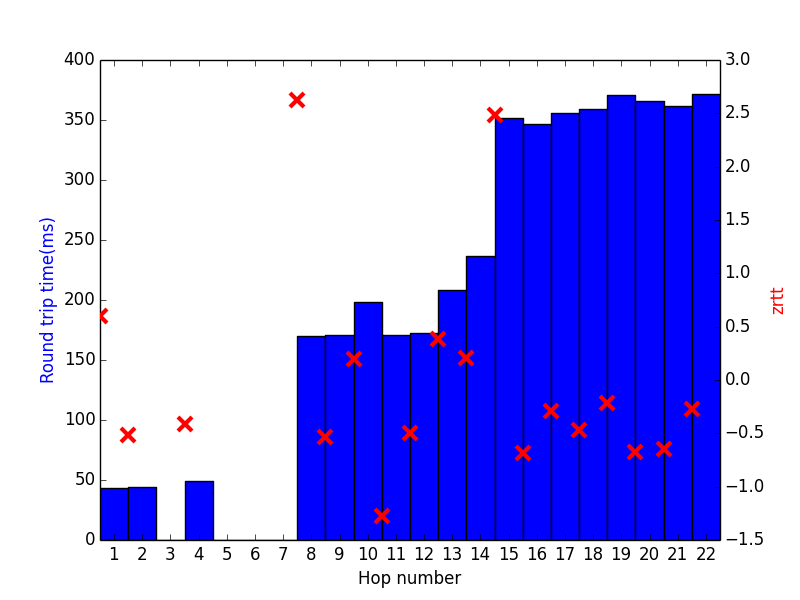
\includegraphics[width=0.5\textwidth]{%
    imagenes/japon.png}
    \caption{Tokyo}
    \label{Tokyo}
\end{center}\end{figure}

\begin{figure}[ht]\begin{center}
   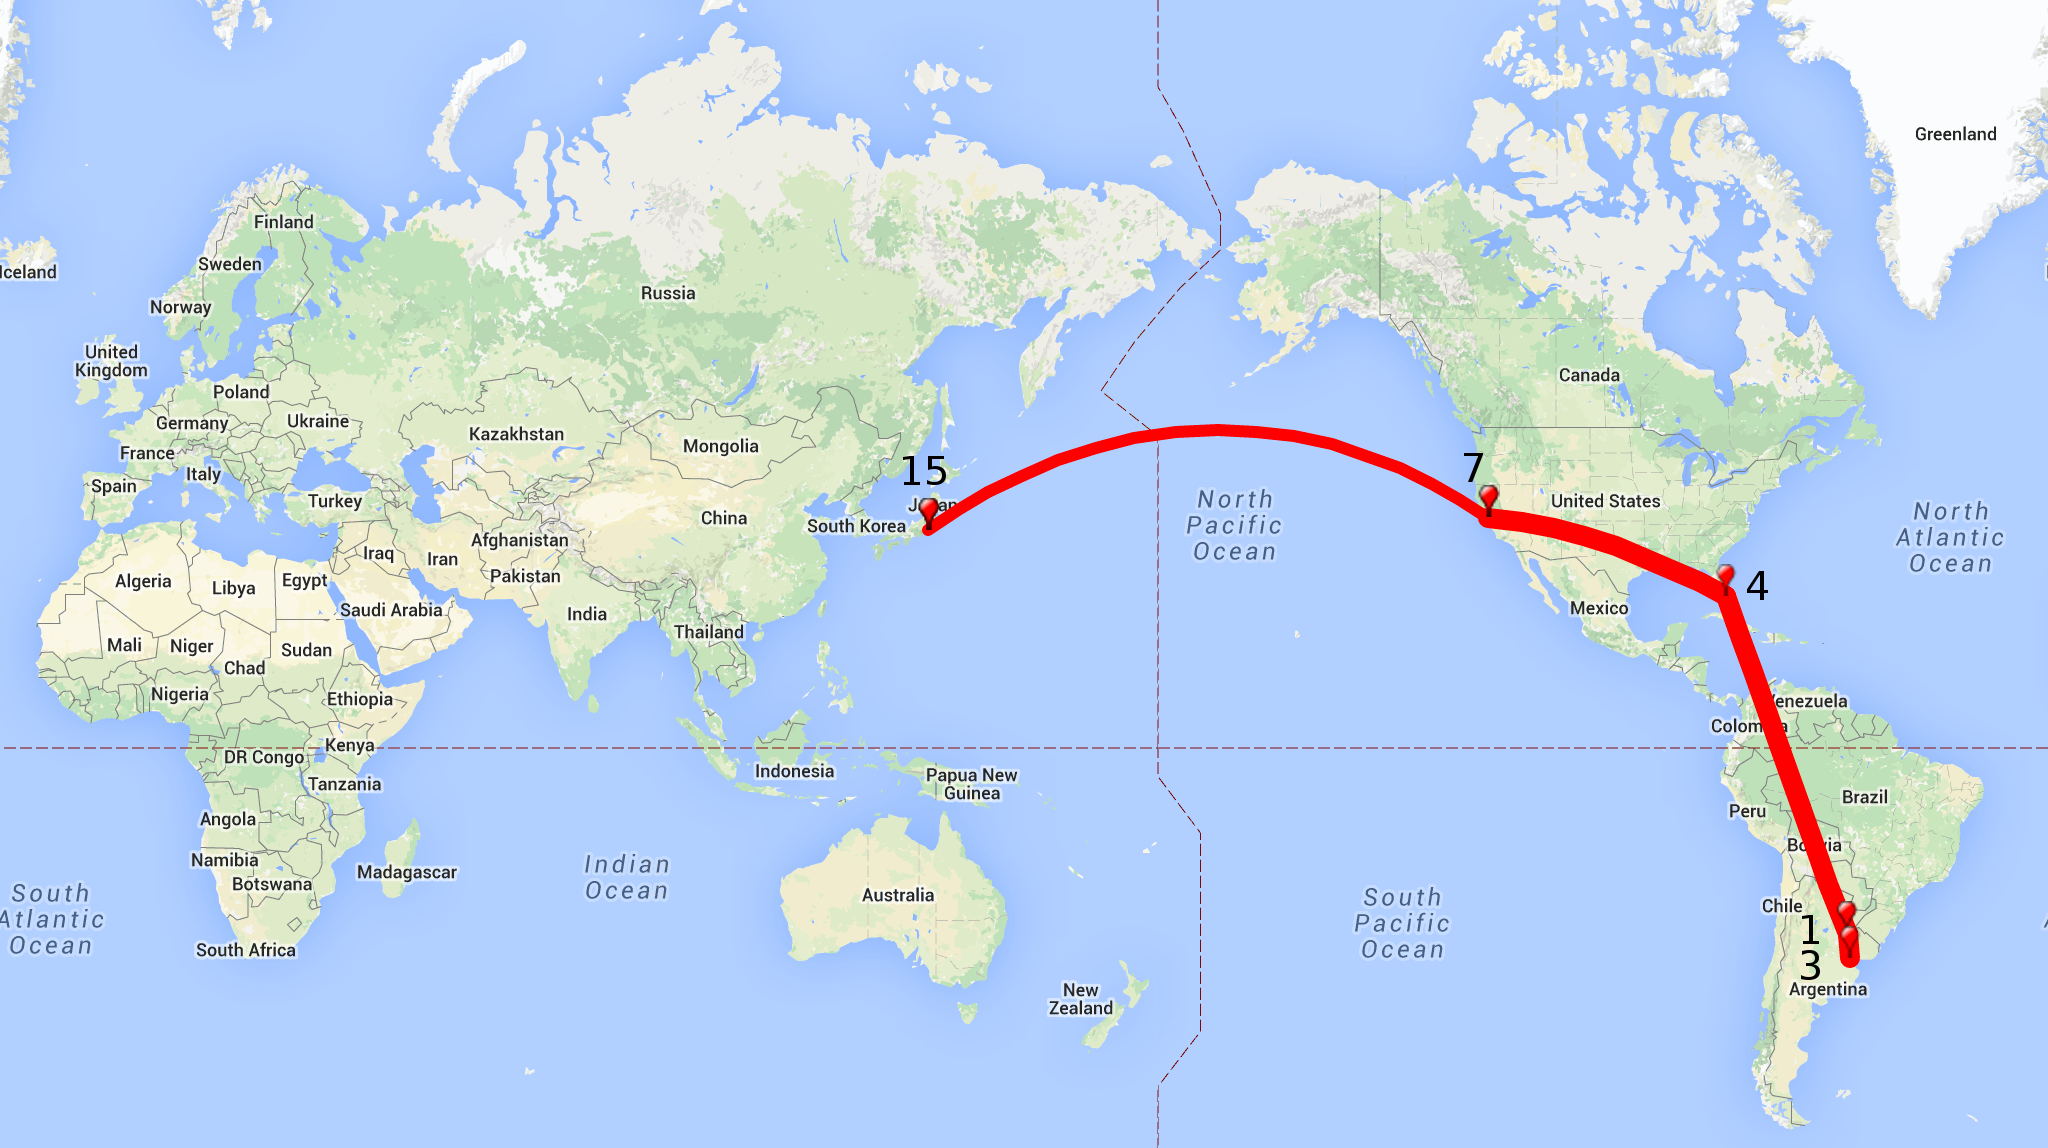
\includegraphics[width=0.5\textwidth]{%
    imagenes/japon-mapa.png}
    \caption{Tokyo - mapa}
    \label{Tokyo}
\end{center}\end{figure}

\subsubsection{Universidad de Oslo}
\begin{figure}[ht]\begin{center}
   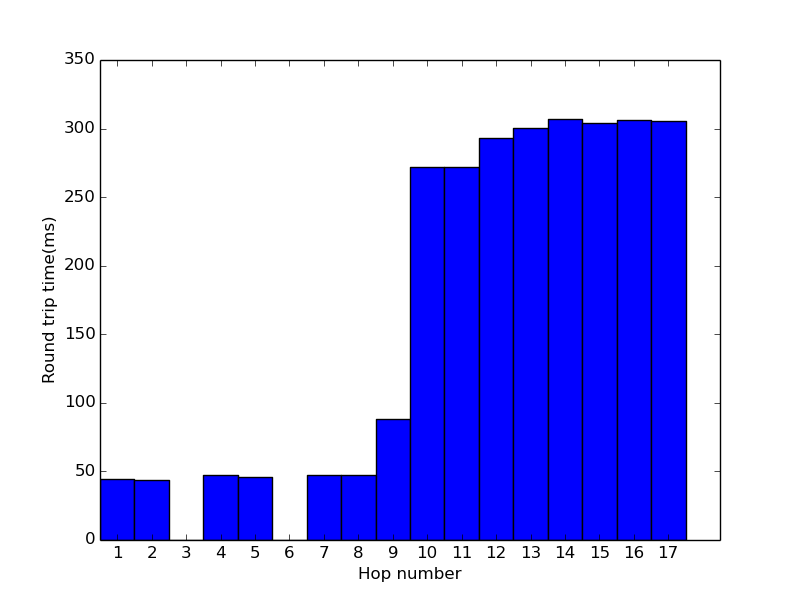
\includegraphics[width=0.5\textwidth]{%
    imagenes/noruega-oslo.png}
    \caption{Noruega}
    \label{Noruega}
\end{center}\end{figure}

\begin{figure}[ht]\begin{center}
   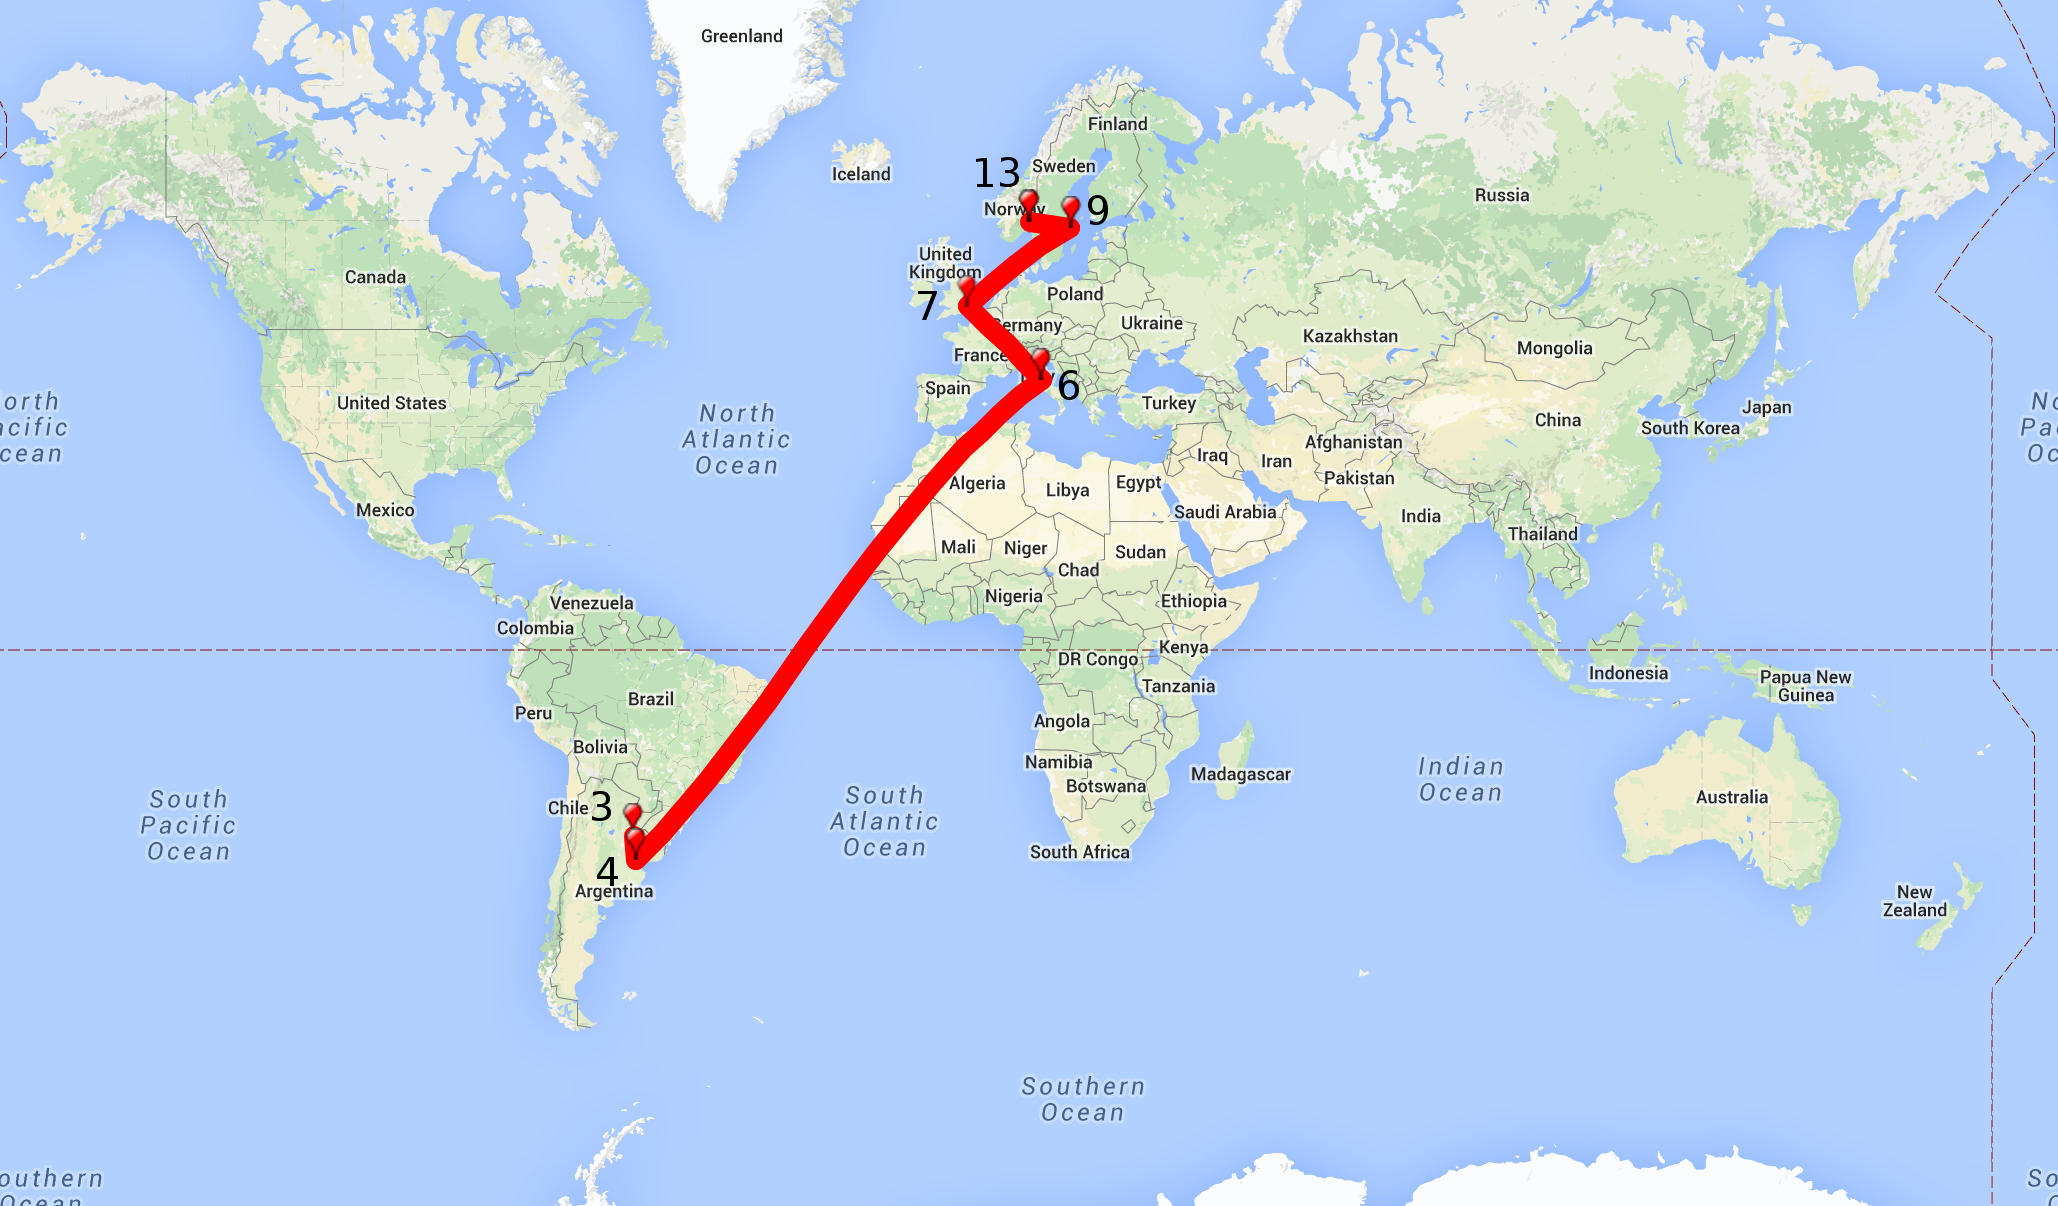
\includegraphics[width=0.5\textwidth]{%
    imagenes/noruega-oslo-mapa.png}
    \caption{Noruega (Oslo) - mapa}
    \label{Noruega}
\end{center}\end{figure}

\subsubsection{Análisis general}
Lo primero que nos llamó la atención de estos histogramas fue que los RTTs observados entre dos
hops consecutivos no siempre son crecientes. Esto en principio no tiene sentido, pues cualquier 
paquete, para llegar al hop $i$, necesariamente debe pasar antes por el hop $i-1$. Luego, 
una posible explicación para esto es que alguno/s router/s de la ruta estén utilizando colas
de prioridad para los paquetes, y que en particular los ICMP (los que nosotros estamos enviando)
tengan una prioridad baja. 

%----------------------------------------------------------------------
% SECTION IV: Contrastando con la realidad
%----------------------------------------------------------------------
\section{Contrastando con la realidad}
A continuación simulamos una conexión mediante sucesivos \emph{pings} (\emph{EchoRequest} $+$ 
\emph{EchoReply}) 
a cada una de las universidades analizadas, y estimamos el \emph{RTT} a dicho destino 
en base a la siguiente ecuación: 
$ EstimatedRTT = \alpha * EstimatedRTT + (1 - \alpha) * SampleRTT $. Con la introducción de
este parámetro $alpha$, lo que haremos es ir actualizando el $EstimatedRTT$ en cada hop del 
recorrido del paquete en función del RTT que hubo en el hop anterior y en el actual, dándoles
un peso (importancia) a cada uno. De esta forma, cuando $alpha$ esté cercano a 0, estaremos
modelando que los RTTs observados entre dos hops consecutivos son bastante independientes,
mientras que si $alpha$ estuviera cercano a 1, querría decir que el RTT observado en un
hop es muy dependiente del RTT observado para el hop anterior. 

Variamos la cantidad de paquetes enviados ($n$) y el $alpha$ para analizar los resultados 
y contrastarlos con los resultados obtenidos en la sección anterior.

Por último, se nos pide que analizemos el eventual $throughput$ punta a punta que se deriva de la
\emph{ecuación de Mathis} para enlaces con pérdida de paquetes estimando la pérdida de la 
siguiente manera:
$EstimatedPacketLossProbability = \dfrac{\#Echo reply}{\#Echo request}$. Aquí hay que aclarar,
que en la ecuación de Mathis asumimos que si $p$ es la probabilidad de pérdida de un paquete,
entonces la cantidad estimada de paquetes enviados exitosamente es $1/p$.





\end{document}












